\documentclass[12pt, letterpaper]{article}
\usepackage[margin=1in]{geometry}
\usepackage{graphicx}
\usepackage{float}
\usepackage[T1]{fontenc}
\usepackage[polish]{babel}
\usepackage[utf8]{inputenc}
\usepackage{amsmath}
\usepackage{listings, newtxtt}
\usepackage{listings}


\graphicspath{{images/}}
\lstset{basicstyle=\ttfamily, keywordstyle=\bfseries, breaklines=true}

\title{Teoria Współbieżności - lab 5 \\ Eliminacja Gaussa}
\author{Błażej Nowicki}
\date{\today}
\begin{document}
\maketitle
\section{Wstęp teoretyczny}
\subsection{Niepodzielne zadania obliczeniowe}

Metoda eliminacji Gaussa jest to algorytm wykorzystywany do m. in.
rozwiązywania układów liniowych. Głównym krokiem jest sprowadzenie macierzy do postaci schodkowej
górnej. Można to osiągnąć odejmując wielokrotności kolejnych wierszy macierzy od wierszy poniżej
aż pod przekątną zostaną same zer.
Mamy daną przykładową macierz z wektorem wyrazów wolnych:

$$
	\begin{bmatrix}
		M_{1,1} & M_{1,2} & M_{1,3} \\
		M_{2,1} & M_{2,2} & M_{2,3} \\
		M_{3,1} & M_{3,2} & M_{3,3} \\
	\end{bmatrix}
	\begin{bmatrix}
		M_{1,4} \\
		M_{2,4} \\
		M_{3,4} \\
	\end{bmatrix}
$$

Można wyróżnić trzy powtarzające się typy operacji:
\begin{itemize}
	\item $ A_{i, k} $ :  $ m_{k,i} = M_{k,i} / M_{i,i} $
	\item $ B_{i,j,k} $: $n_{k,i,j} = M_{i,j} * m_{k,i} $
	\item $ C_{i,j,k} $ :  $ M_{k,j} = M_{k,j} - n_{k,i,j} $
\end{itemize}

\subsection{Ciąg operacji}

Analizując jakie kroki należy wykonać można zauważyć powtarzający się schemat.
Dla każdego  wiersza najpierw wyznaczamy współczynnik - operacja $A$, a następnie
na zmianę  $B$ i $C$ dla każdej kolumny. Efektywnie odejmujemy jeden wiersz od drugiego z wyznaczonym współczynnikiem. \\
Można tą operację oznaczyć jako $p_{i,k}$, gdzie: \\
$ p_{i,k} $ - odjęcie i-tego wiersza od k-tego ze współczynnikiem $M_{k,i}/M_{i,i}$ \\
$ p_{i,k} = ( A_{i,k}, B_{i,i,k}, C_{i,i,k}, B_{i,i+1,k}, C_{i,i+1,k},\ldots,B_{i, s+1, k}, C_{i,s+1,k}) $ \\
$s$ - rozmiar macierzy \\
Wtedy ciąg wszystkich operacji można zapisać jako: \\
$ (p_{1,2}, p_{1,3}, \ldots, p_{1,s},\\
	p_{2,3}, p_{2,3}, \ldots, p_{2, s},\\
	\ldots\\
	p_{s-2, s-1}, p_{s-2, s} \\
	p_{s-1, s}
	) $

\subsection{Alfabet}

$ \Sigma = \{ A_{i,k} | i \subseteq \{1, \ldots, s-1\}, k \subseteq \{ i+1, \ldots, s \}\} \cup \\
	\{ B_{i,j,k} | i \subseteq \{1, \ldots, s-1\}, k \subseteq \{ i+1, \ldots, s \}, j \subseteq \{ i, \ldots, s+1 \}\} \cup \\
	\{ C_{i,j,k} | i \subseteq \{1, \ldots, s-1\}, k \subseteq \{ i+1, \ldots, s \}, j \subseteq \{ i, \ldots, s+1 \}\}$

\subsection{Relacja zależności}

Relacja zależności jest wyznaczana dynamicznie podczas działania programu. \\
Przykładowy wynik działania programu dla macierzy rozmiaru 3 przy przyjętych powyżej definicjach.

\begin{lstlisting}
D = {(A12,A12),(A12,B112),(A12,B122),(A12,B132),(A12,B142),(A12,C112),(A13,A13),(A13,B113),(A13,B123),(A13,B133),(A13,B143),(A13,C113),(A23,A23),(A23,B223),(A23,B233),(A23,B243),(A23,C122),(A23,C123),(A23,C223),(B112,A12),(B112,B112),(B112,C112),(B113,A13),(B113,B113),(B113,C113),(B122,A12),(B122,B122),(B122,C122),(B123,A13),(B123,B123),(B123,C123),(B132,A12),(B132,B132),(B132,C132),(B133,A13),(B133,B133),(B133,C133),(B142,A12),(B142,B142),(B142,C142),(B143,A13),(B143,B143),(B143,C143),(B223,A23),(B223,B223),(B223,C122),(B223,C223),(B233,A23),(B233,B233),(B233,C132),(B233,C233),(B243,A23),(B243,B243),(B243,C142),(B243,C243),(C112,A12),(C112,B112),(C112,C112),(C113,A13),(C113,B113),(C113,C113),(C122,A23),(C122,B122),(C122,B223),(C122,C122),(C123,A23),(C123,B123),(C123,C123),(C123,C223),(C132,B132),(C132,B233),(C132,C132),(C133,B133),(C133,C133),(C133,C233),(C142,B142),(C142,B243),(C142,C142),(C143,B143),(C143,C143),(C143,C243),(C223,A23),(C223,B223),(C223,C123),(C223,C223),(C233,B233),(C233,C133),(C233,C233),(C243,B243),(C243,C143),(C243,C243)}
\end{lstlisting}

\subsection{Graf zależności Diekerta}

Graf zależności i jedgo minimalizacja jest realizowana dynamicznie podczas działania programu. Poniżej przedstawiono przykładowy wynik działania programu dla macierzy rozmiaru 3

\begin{figure}[h]
	\centering
	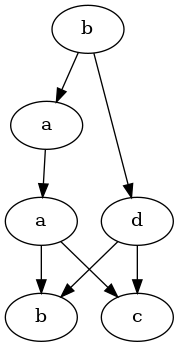
\includegraphics[width=\textwidth]{graph.png}
	\caption{Wygenerowany graf zależności operacji przy eliminacji Gaussa}
\end{figure}

\subsection{Klasy Foaty}

Klasy Foaty są automatycznie wyznaczane poprzez kolorowanie grafu z usuniętymi przechodnimi krawędziami. Przykład dla grafu z poprzedniego podpunktu.

\begin{lstlisting}
	FNF([w]) = (A12,A13)(B112,B122,B132,B142,B113,B123,B133,B143)(C112,C122,C132,C142,C113,C123,C133,C143)(A23)(B223,B233,B243)(C223,C233,C243)
\end{lstlisting}

\section{Implementacja}
% \texttt{}
W celu implementacji skorzystano z języka Python.
Zdefiniowano klasy reprezentujące obiekty: produkcję, relację, graf i postać normalną Foaty.

Klasa abstrakcyjna \texttt{Task} określa podstawowe zachowanie niepodzielnego zadania obliczeniowego.
Zawiera nazwę zadania, z jakich symboli korzysta na wejściu i jakie symbole modyfikuje. Pozwala na wyznaczenie relacji zależności.
$ A_{i,k} $, $B_{i,j,k}$ i $ C_{i,j,k} $ dziedziczą po Task i przeciążają motodę \texttt{run}, która wykonuje operacje na współdzielonych danych.

\texttt{Relation} wyznacza relację zależności na podstawie definicji. Zadania są wzajemnie zależne jeśli zmienna modyfikowana przez jedno pojawia się na wejściu lub wyjściu drugiej.

\texttt{Graph} konstruuje graf zależności na podstawie przekazanej relacji i słowa nad alfabetem składającego się ze wszystkich operacji.
Przeprowadzane jest usuwanie przechodnich krawędzi.
Zastosowano algorytm oparty na obserwacji że dane zadanie będące w słowie przed innym zadaniem nie może być od niego zależne.
Dla każdego wierzchołka zapisywane jest lista wszystkich zadań które muszą zostać wykonane przed nim.
Jeśli dodanie krawędzi z pomiędzy dwoma zależnymi zadaniami nie powiększa tej listy to znaczy że krawędź jest zbędna.
Wyznaczanie klas Foaty zrealizowano analogicznie do algorytmu kolorowania grafu.
(Szczegóły opisano w kodzie)


\texttt{Scheduler} przyjmuje jako argument zadania podzielone na klasy Foaty.
Tworzy pule wątków dla każdej klasy i wykonuje obliczenia w omawianym przypadku na trzech współdzielonych tablicach \texttt{M}, \texttt{n}, \texttt{m}.

\end{document}